\section{Red oficina}

Para este experimento se tomo una captura de 30 minutos de la red Wi-Fi la oficina de taringa.
La oficina al momento de la captura contaba con unas 20 personas conectadas a la red.
En esta captura se filtró previamente los paquetes ARP antes de ser procesados para el analisis,
por lo tanto los resultados son un poco distintos.

\begin{figure}[H]
  \centering
    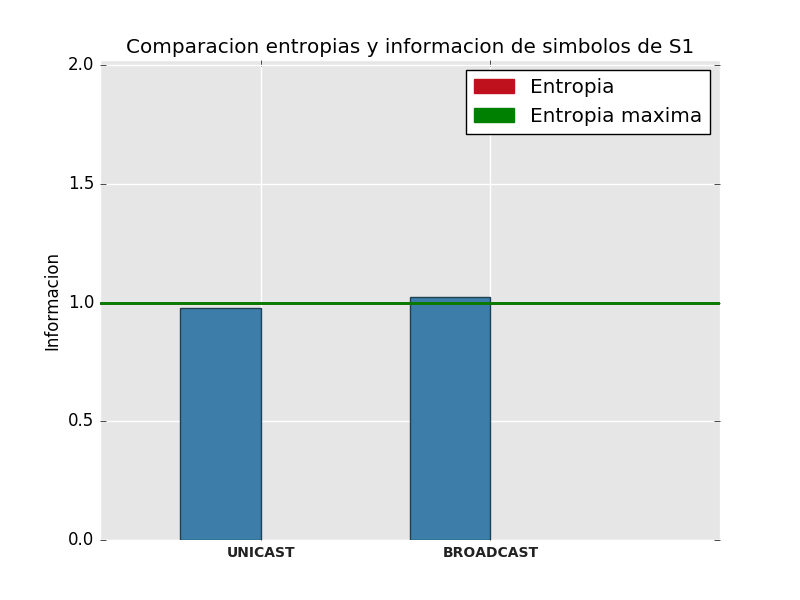
\includegraphics[width=0.45\textwidth]{grafico1-red-taringa.png}
  \caption{Entropia de la fuente}
  \label{entropia-taringa-1}
\end{figure}

Como se puede ver en el gráfico, la entropía llega a ser casi máxima (0,999). 
Esto es debido a que se capturó casi la misma cantida de paquetes UNICAST como de BROADCAST
por lo tanto un símbolo UNICAST proporciona la misma información que un símbolo BROADCAST 

\begin{figure}[H]
  \centering
    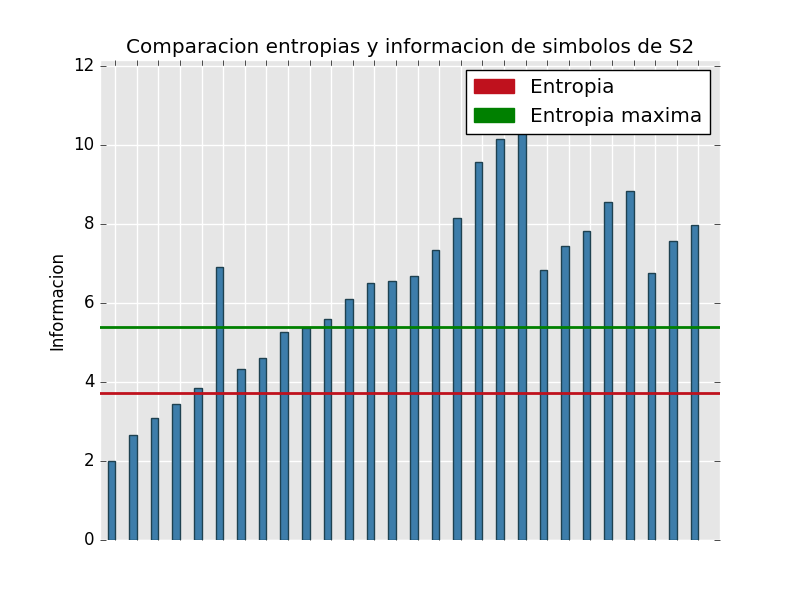
\includegraphics[width=0.45\textwidth]{grafico2-red-taringa.png}
  \caption{Entropia de la fuente}
  \label{entropia-taringa-2}
\end{figure}

    \begin{table}[ht]\begin{center}
      \begin{tabular}{|c|c|}
      \hline
      \textbf{Nodo} & \textbf{Informacion} \\ \hline
      \texttt{192.168.1.224 }& 1.987991 \\ \hline
      \texttt{192.168.1.211 }& 2.666566 \\ \hline
      \texttt{192.168.1.1}& 3.089686 \\ \hline
      \texttt{192.168.1.243}& 3.436136 \\ \hline
      \end{tabular}
      \caption{Nodos destacados}
      \label{Nodos-destacados-taringa}
    \end{center}\end{table}

Lo mas probable es que el nodo 192.168.1.1 sea el Default Gateway por la cantidad de información que posee
y además por intuición en su dirección ip, 
Es probable que los demás nodos sean servidores que servicios utilizados por procesos en algún otro host.

\begin{figure}[H]
  \centering
    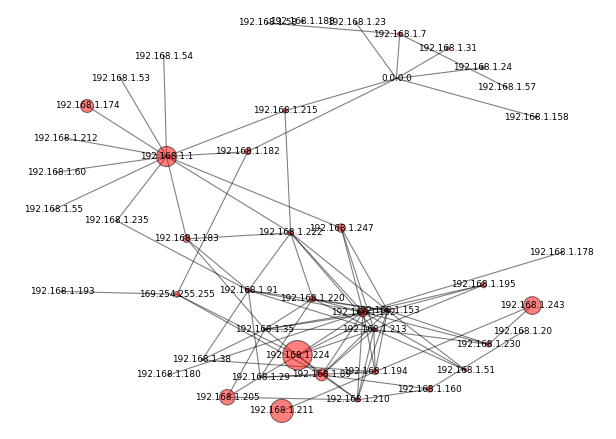
\includegraphics[width=0.45\textwidth]{grafico3-red-taringa.png}
  \caption{Grafo de la red}
  \label{grafo-taringa}
\end{figure}
